\documentclass[12pt, letterpaper]{article}
\usepackage{bookmark}
\usepackage{graphicx}
\usepackage{hyperref}
\usepackage{xcolor}

\title{SENG 474 A02: Assignment 2 \\[1ex]
\large Model Selection Experiments:
\large \textit{Logistic Regression, Support Vector Machines, and k-Fold Cross Validation}}
\author{Sean McAuliffe, V00913346 }
\date{February 27th, 2023}
\graphicspath{{./figures/}}

\begin{document}

\maketitle

\pagebreak
\tableofcontents  
\pagebreak

\section{Background}

\paragraph*{}This report summarizes the results of a series of experiments
conducted which implement two methods for binary classification: Logistic
Regression, and Support Vector Machines (SVM). The purpose of this exercise
was to compare the performance of these two methods, as well as to practice
the use of cross-entropy loss and \textit{k}-Fold Cross Validation for
selection of optimal model hyperparameters. 

\paragraph*{}For each of these approaches a number of models were trained on
the Fashion-MNIST
\href{github.com/zalandoresearch/fashion-mnist}{\textcolor{blue}{\underline{dataset}}}.
The Fashion-MNIST dataset is a collection of 70,000 grayscale 28x28 pixel images of
clothing items in 10 classes. For the purposes of these experiments, only
classes 0 and 6 (T-shirt and Shirt) were used. Furthermore, to reduce runtimes
during SVM training, only 2,400 training images, and 2000 testing images were used
throughout the experiments.

\section{Environment and Implementation}

\paragraph*{}Linear Regression and SVM implementation from \textbf{scikit-learn}
were used for this assignment. Of note for this report, the \textbf{scikit-learn}
library implements the \textit{linear\_model.LinearRegression} and \textit{svm.SVC}
classes for Logistic Regression and SVM, respectively. These classes were used
to train and test the models for this assignment. 

\paragraph*{}All code for this assignment, including data import, preprocessing
model creation, training, evluation and plot generation was done in Jupyter
Notebooks running on a \textbf{Python 3.10.6} kernel. Relying on utility
functions provided with the Fashion-MNIST dataset, the source code for which
has been provided with included with the .ipynb files with this report.

\section{\textit{k}-Fold Cross Validation}

\paragraph*{}The \textit{k}-Fold Cross Validation method is an improvement
on the simple cross-validation which was used to evaluate model performance
in the previous assignment. Cross validation involves splitting the available
data into training and validation sets; models will be trained on the training
set, and scored against the valdiation set. In this way the true risk of the
model can be estimated on data which was not used to train the model.

\begin{figure}[ht]
    \centering
    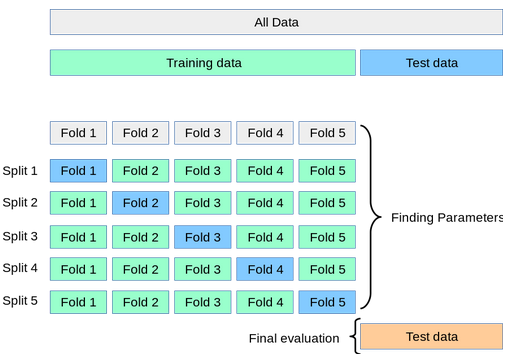
\includegraphics[width=0.75\textwidth]{0.png}
    \caption{k-fold cross validation method, source \href{https://scikit-learn.org/stable/modules/cross_validation.html}{\textcolor{blue}{\underline{scikit-learn.org}}}}
    \label{fig:1}
\end{figure}

\paragraph*{}The \textit{k}-Fold Cross Validation method is a better way to
evaluate model performance. It is more robust to the choice of training and
validation sets, and is more computationally efficient than the simple
method. The \textit{k}-Fold Cross Validation method involves splitting the
available data into \textit{k} equal sized subsets. Then for each \textit{i}
between 0 and \textit{k}-1, the model is trained on all subsets except the
\textit{ith} subset, and evaluated on the \textit{ith} subset. The average
performance of the model across all \textit{k} iterations is reported as the
model accuracy. 

\paragraph*{}The intended use of this method is to evaluate the difference in
model performance as hyperparemeters are varied, in order to choose the optimal
hyperperameters for the context, without leaking information from the validation set.
In this method, the final test data set is only consulted after the hyperparameters
have been chosen. The implementation used in this assignment is shown below.

\begin{verbatim}
def kfold_cv(X, y, k, model):
  # Split the data into k folds
  X_folds = np.array_split(X, k)
  y_folds = np.array_split(y, k)
  accuracies = []
  for i in range(k):
    # Create training and validation sets
    # Training sets contain every fold except the ith
    X_train = np.concatenate(X_folds[:i] + X_folds[i+1:])
    y_train = np.concatenate(y_folds[:i] + y_folds[i+1:])
    # Validation set is the ith fold
    X_validation = X_folds[i]
    y_validation = y_folds[i]
    # Train the model
    model.fit(X_train, y_train)
    # Evaluate the model
    accuracies.append(model.score(X_validation, y_validation))
  return 1 - np.average(np.array(accuracies))
\end{verbatim}

\paragraph*{}A small (and likely unrepresentative) experiment was conducted
to choose a value for \textit{k} to use in this assigmnent. A Logistic Regression
model, using the default parameters was trained on the Fashion-MNIST dataset
and scored against the test set; the score was computed using the \textit{k}-Fold
Cross Validation implementation above with \textit{k} ranging from 5 to 10.
The results of this experiment are shown in Figure \ref{fig:3}. Since there was
no siginficant difference in outcome between the values of \textit{k} tested,
the value of 5 was chosen for the remainder of the experiments to reduce runtime.

\begin{figure}[ht]
    \centering
    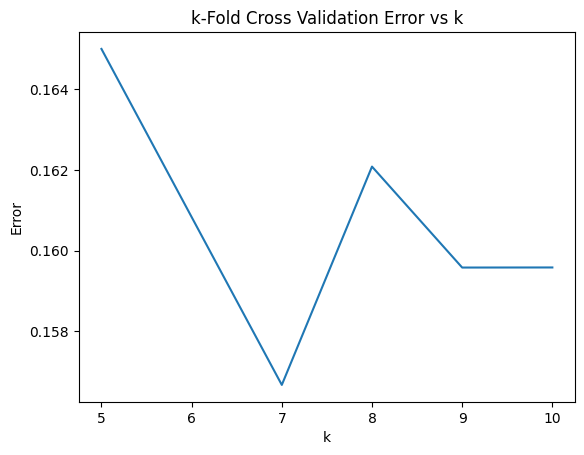
\includegraphics[width=0.75\textwidth]{1.png}
    \caption{LR Model Error vs. k}
    \label{fig:3}
\end{figure}

\section{Logistic Regression}



\end{document}